\section{Introduction}
\label{sec:intro}

\begin{wrapfigure}{R}{0.55\textwidth}
    \vspace{-3mm}

    \centering
    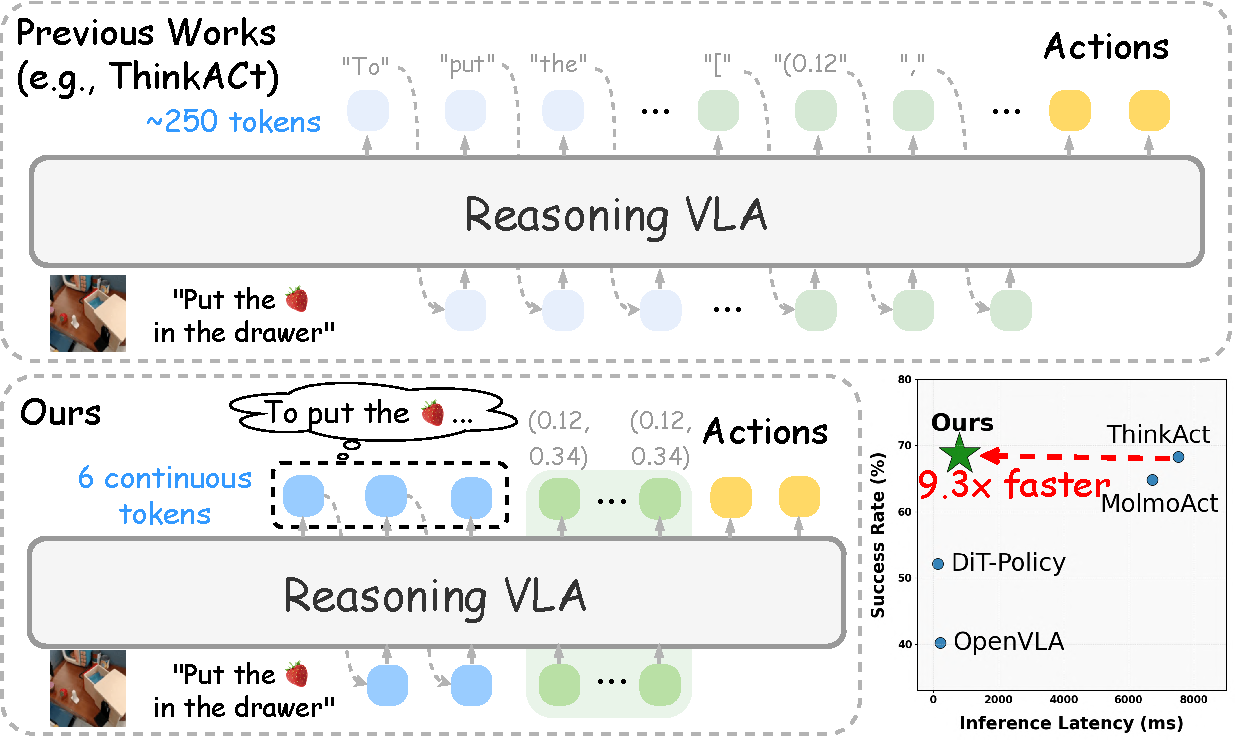
\includegraphics[width=1.0\linewidth]{figures/images/teaser.pdf}

    \vspace{1.5mm}
    
    \caption{\textbf{Overview of \ours{}.} Previous reasoning VLAs generate lengthy reasoning traces ($\sim$250 tokens). Our approach learns compact continuous tokens (e.g., 6) (\textcolor{cyan}{blue}) and parallel spatial tokens (\textcolor{YellowGreen}{green}) as internal reasoning. The bottom-right plot shows that we achieve $9.3\times$ faster inference than ThinkAct-7B~\cite{huang2025thinkact}, while delivering improved performance on the SimplerEnv-Google benchmark.}
    \label{fig:teaser}
\end{wrapfigure}



Recent large vision-language models (VLMs)~\cite{liu2023visual,comanici2025gemini,liu2024nvila,bai2025qwen2,shi2024eagle,li2025eagle,chen2025eagle,wang2025internvl3,xie2024show} have achieved remarkable capabilities in visual-language understanding across diverse multimodal tasks. To extend these capabilities to embodied-centric tasks, recent works leverage large-scale robot demonstrations~\cite{o2024open} to develop Vision-Language-Action (VLA) foundation models~\cite{brohan2022rt,brohan2023rt,team2024octo,bjorck2025gr00t,li2025hamster,black2024pi_0,yang2025magma,kim24openvla}. These VLA tasks require agents to perceive complex visual scenes, reason over spatial and temporal contexts, and execute adaptive actions within dynamic environments, demanding robust long-horizon planning and contextual adaptation. However, as these VLA models primarily rely on supervised training from action data, they excel at basic skills (e.g., pick-and-place) but struggle to generalize beyond training distributions, such as long-horizon planning, self-correction from failures, and adaptation to novel scenarios, due to the impracticality of collecting exhaustive robot demonstrations.


Reasoning VLAs~\cite{zawalski2024robotic,zhao2025cot,lee2025molmoact,wu2025you,qu2025eo,huang2025thinkact,kim2025robot} address these limitations by incorporating intermediate thinking processes, improving generalization and task-solving capability. Supervised chain-of-thought (CoT) methods~\cite{zawalski2024robotic,zhao2025cot,lee2025molmoact,qu2025eo} address this by learning from intermediate reasoning annotations. These approaches can be categorized into textual reasoning methods that leverage off-the-shelf LLMs and VLMs to generate pseudo CoT labels~\cite{zawalski2024robotic}, and visual reasoning methods that generate structured visual reasoning representations such as sub-goal images, image depth, and 2D visual traces~\cite{zhao2025cot,lee2025molmoact}. However, these supervised approaches require substantial reasoning annotations and remain limited by training data coverage. To address this, ThinkAct~\cite{huang2025thinkact} employs RL-based reasoning~\cite{shao2024deepseekmath} to generate long textual CoTs guided by action-aligned visual rewards. While these reasoning methods effectively improve task generalization and planning capabilities, they require generating lengthy chain-of-thought steps that introduce substantial reasoning latency, which hampers embodied applications with \emph{real-time} requirements.


In embodied AI applications such as robotic manipulation and autonomous driving, agents must make rapid decisions at high frequencies (e.g., 1-15 Hz)~\cite{guan2025efficient}. However, generating lengthy reasoning traces can take several seconds per decision (e.g., 0.1 Hz)~\cite{huang2025thinkact, lee2025molmoact}, creating a critical bottleneck that limits real-time performance~\cite{guan2025efficient, yu2025survey} and poses safety risks in time-critical scenarios~\cite{wang2025alpamayo}. To mitigate this efficiency bottleneck while preserving reasoning capabilities, very recent works~\cite{chen2025training, yu2025survey, guan2025efficient} have explored approaches to reduce inference latency in embodied reasoning. For instance, ECoT-Lite~\cite{chen2025training} proposes reasoning dropout to accelerate inference, yet directly reducing textual reasoning length risks performance degradation due to critical information loss. How to preserve reasoning capability while enabling compact representations that properly capture essential spatial-temporal dynamics remains a crucial challenge for reasoning VLA models.



In this paper, we propose \textit{\ours{}}, an efficient embodied reasoning framework for Vision-Language-Action tasks that achieves compact yet expressive planning through verbalizable latent reasoning. As depicted in Figure~\ref{fig:teaser}, unlike prior reasoning VLAs that generate lengthy explicit textual CoT traces, we introduce reward-guided preference distillation with visual trajectory alignment to compress linguistic and visual planning into compact continuous latents that enable implicit internal reasoning. Our student VLM encodes reasoning into compact latents decodable by a verbalizer, enabling preference-based optimization that leverages RL-derived reward signals to distill high-quality reasoning patterns from a textual teacher VLM while suppressing low-quality ones. We further align trajectory latents between teacher and student to transfer visual planning capabilities essential for embodied control. Once trained, the student VLM enables reasoning-enhanced policy learning that bridges implicit multimodal planning with action execution, achieving significantly faster inference while outperforming existing reasoning VLAs.



Our contributions can be summarized as follows:
\begin{itemize}
    \item We propose \textit{\ours{}}, an efficient reasoning framework that compresses reasoning into verbalizable latent thoughts while maintaining expressive planning abilities.
    
    \item We introduce preference-guided distillation with manipulation trajectory alignment that compresses linguistic and visual planning into compact continuous latents.
    
    \item We bridge high-level visual planning to low-level action execution through reasoning-enhanced policy learning guided by manipulation trajectory latents.
    
    \item We achieve up to 89.3\% inference latency reduction over state-of-the-art reasoning VLAs while maintaining strong performance across diverse embodied benchmarks.
\end{itemize}